\section{AM SSB}

\begin{frame}{AM SSB: A Motivação}

\only<1>{
\textbf{Observação fundamental no DSB-SC:}

\begin{center}
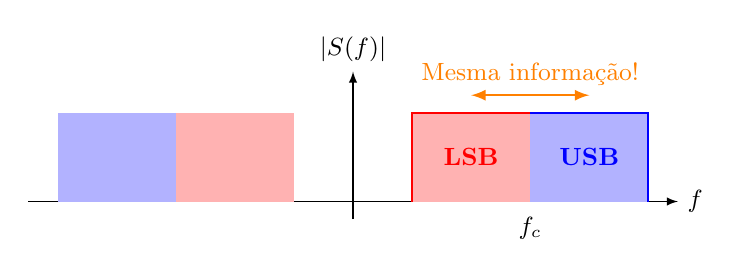
\begin{tikzpicture}[>=latex, scale=0.75]
\draw[->] (-5.5,0) -- (5.5,0) node[right, font=\small] {$f$};
\draw[->] (0,-0.3) -- (0,2.2) node[above, font=\small] {$|S(f)|$};
% USB e LSB
\fill[red!30] (1,0) -- (1,1.5) -- (3,1.5) -- (3,0) -- cycle;
\fill[blue!30] (3,0) -- (3,1.5) -- (5,1.5) -- (5,0) -- cycle;
\draw[thick, red] (1,0) -- (1,1.5) -- (3,1.5);
\draw[thick, blue] (3,1.5) -- (5,1.5) -- (5,0);
\fill[blue!30] (-5,0) -- (-5,1.5) -- (-3,1.5) -- (-3,0) -- cycle;
\fill[red!30] (-3,0) -- (-3,1.5) -- (-1,1.5) -- (-1,0) -- cycle;
\node[font=\small, red] at (2,0.75) {\textbf{LSB}};
\node[font=\small, blue] at (4,0.75) {\textbf{USB}};
\node[below, font=\small] at (3,-0.1) {$f_c$};
\draw[<->, thick, orange] (2,1.8) -- (4,1.8) node[midway, above, font=\small] {Mesma informação!};
\end{tikzpicture}
\end{center}

\textbf{LSB e USB carregam informação idêntica} $\rightarrow$ Redundância!

\textbf{Ideia:} Transmitir apenas \textbf{uma} banda lateral $\rightarrow$ economia de 50\%
}

\only<2>{
\textbf{SSB remove uma banda lateral:}

\begin{center}
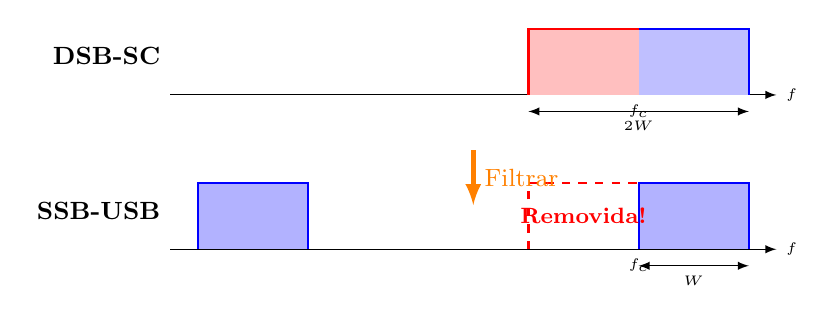
\begin{tikzpicture}[>=latex, scale=0.7]
% DSB-SC
\begin{scope}[yshift=1.8cm]
\node[left, font=\small\bfseries] at (-5.5,0.7) {DSB-SC};
\draw[->] (-5.5,0) -- (5.5,0) node[right, font=\tiny] {$f$};
\fill[red!25] (1,0) -- (1,1.2) -- (3,1.2) -- (3,0) -- cycle;
\fill[blue!25] (3,0) -- (3,1.2) -- (5,1.2) -- (5,0) -- cycle;
\draw[thick, red] (1,0) -- (1,1.2) -- (3,1.2);
\draw[thick, blue] (3,1.2) -- (5,1.2) -- (5,0);
\node[below, font=\tiny] at (3,0) {$f_c$};
\draw[<->] (1,-0.3) -- (5,-0.3) node[midway, below, font=\tiny] {$2W$};
\end{scope}
% SSB-USB
\begin{scope}[yshift=-1cm]
\node[left, font=\small\bfseries] at (-5.5,0.7) {SSB-USB};
\draw[->] (-5.5,0) -- (5.5,0) node[right, font=\tiny] {$f$};
\fill[blue!30] (3,0) -- (3,1.2) -- (5,1.2) -- (5,0) -- cycle;
\draw[thick, blue] (3,0) -- (3,1.2) -- (5,1.2) -- (5,0);
\fill[blue!30] (-5,0) -- (-5,1.2) -- (-3,1.2) -- (-3,0) -- cycle;
\draw[thick, blue] (-5,0) -- (-5,1.2) -- (-3,1.2) -- (-3,0);
\node[below, font=\tiny] at (3,0) {$f_c$};
\draw[<->] (3,-0.3) -- (5,-0.3) node[midway, below, font=\tiny] {$W$};
\node[font=\footnotesize, red] at (2,0.6) {\textbf{Removida!}};
\draw[thick, red, dashed] (1,0) -- (1,1.2) -- (3,1.2);
\end{scope}
% Seta
\draw[->, ultra thick, orange] (0,0.8) -- (0,-0.2) node[midway, right, font=\small] {Filtrar};
\end{tikzpicture}
\end{center}

$B_{\text{SSB}} = W$ \quad (metade do DSB!) \quad Economia de 50\% em banda
}

\end{frame}

% ============================================

\begin{frame}{SSB: Vantagens, Desvantagens e Aplicações}

\begin{columns}[T]
\begin{column}{0.48\textwidth}
\onslide<1->{
\textbf{Vantagens:}
\begin{itemize}
\item $B = W$ (metade do DSB)
\item Potência concentrada
\item Menos interferência
\end{itemize}
}

\onslide<2->{
\textbf{Desvantagens:}
\begin{itemize}
\item Geração complexa
\item Detecção coerente
\item Sensível a erro de $\Delta f$
\end{itemize}
}
\end{column}
\begin{column}{0.50\textwidth}
\onslide<3->{
\textbf{Aplicações:}
\begin{itemize}
\item Rádio amador (HF: 3--30 MHz)
\item Comunicações marítimas
\item Militar (longa distância)
\end{itemize}

\vspace{0.3cm}

\begin{center}
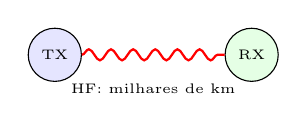
\begin{tikzpicture}[>=latex, scale=0.5]
% Mapa mundo simplificado
\node[draw, circle, fill=blue!10, minimum size=0.6cm, font=\tiny] (tx) at (0,0) {TX};
\node[draw, circle, fill=green!10, minimum size=0.6cm, font=\tiny] (rx) at (5,0) {RX};
\draw[thick, red, decorate, decoration={snake, amplitude=2pt, segment length=8pt}] (tx) -- (rx);
\node[below, font=\tiny] at (2.5,-0.5) {HF: milhares de km};
\end{tikzpicture}
\end{center}
}
\end{column}
\end{columns}

\end{frame}

% ============================================

\begin{frame}{Representação Matemática do SSB}

\only<1>{
\textbf{Como gerar SSB?} Duas abordagens:

\vspace{0.3cm}

\begin{center}
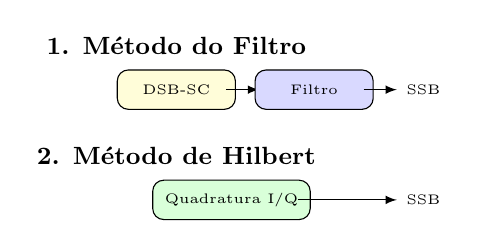
\begin{tikzpicture}[>=latex, scale=0.7]
% Método 1
\begin{scope}[yshift=1.2cm]
\node[font=\small\bfseries] at (0,0.8) {1. Método do Filtro};
\node[draw, rectangle, fill=yellow!15, rounded corners, minimum width=1.5cm, minimum height=0.5cm, font=\tiny] (m1) at (0,0) {DSB-SC};
\draw[->] (0.9,0) -- (1.5,0);
\node[draw, rectangle, fill=blue!15, rounded corners, minimum width=1.5cm, minimum height=0.5cm, font=\tiny] (f1) at (2.5,0) {Filtro};
\draw[->] (3.4,0) -- (4,0) node[right, font=\tiny] {SSB};
\end{scope}
% Método 2
\begin{scope}[yshift=-0.8cm]
\node[font=\small\bfseries] at (0,0.8) {2. Método de Hilbert};
\node[draw, rectangle, fill=green!15, rounded corners, minimum width=2cm, minimum height=0.5cm, font=\tiny] (m2) at (1,0) {Quadratura I/Q};
\draw[->] (2.2,0) -- (4,0) node[right, font=\tiny] {SSB};
\end{scope}
\end{tikzpicture}
\end{center}
}

\only<2>{
\textbf{Resultado usando Transformada de Hilbert:}

\vspace{0.3cm}

\textbf{SSB-USB:}
\[
\boxed{s_{\text{USB}}(t) = \frac{A_c}{2}[m(t)\cos(2\pi f_c t) - \hat{m}(t)\sin(2\pi f_c t)]}
\]

\textbf{SSB-LSB:}
\[
\boxed{s_{\text{LSB}}(t) = \frac{A_c}{2}[m(t)\cos(2\pi f_c t) + \hat{m}(t)\sin(2\pi f_c t)]}
\]

onde $\hat{m}(t)$ é a \textbf{transformada de Hilbert} de $m(t)$

\vspace{0.2cm}

O sinal $-$ cancela a LSB (sobra USB). O sinal $+$ cancela a USB (sobra LSB)
}

\end{frame}

% ============================================

\begin{frame}{Transformada de Hilbert}

\only<1>{
\textbf{Definição no tempo:}
\[
\hat{m}(t) = m(t) \ast \frac{1}{\pi t} = \frac{1}{\pi} \int_{-\infty}^{\infty} \frac{m(\tau)}{t - \tau}\, d\tau
\]

\textbf{Definição na frequência:}
\[
\hat{M}(f) = -j\,\sgn(f)\, M(f) = \begin{cases}
-jM(f) & f > 0 \\
+jM(f) & f < 0
\end{cases}
\]

\textbf{Interpretação:} defasador de $-90^{\circ}$ para todas as frequências
}

\only<2>{
\textbf{Exemplos com tom único:}

\vspace{0.3cm}

\begin{columns}[T]
\begin{column}{0.45\textwidth}
$\hat{\cos}(2\pi ft) = \sin(2\pi ft)$

$\hat{\sin}(2\pi ft) = -\cos(2\pi ft)$
\end{column}
\begin{column}{0.53\textwidth}
\begin{center}
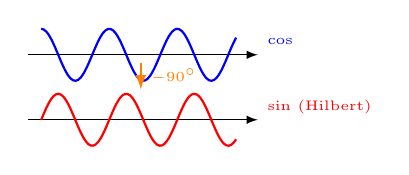
\begin{tikzpicture}[>=latex, scale=0.55]
% cos
\draw[->] (-0.3,0) -- (5,0);
\draw[thick, blue, smooth] plot[domain=0:4.5, samples=80] (\x, {0.6*cos(4*\x r)});
\node[right, font=\tiny, blue] at (5,0.3) {$\cos$};
% sin (Hilbert de cos)
\begin{scope}[yshift=-1.5cm]
\draw[->] (-0.3,0) -- (5,0);
\draw[thick, red, smooth] plot[domain=0:4.5, samples=80] (\x, {0.6*sin(4*\x r)});
\node[right, font=\tiny, red] at (5,0.3) {$\sin$ (Hilbert)};
\end{scope}
% Seta
\draw[->, thick, orange] (2.3,-0.2) -- (2.3,-0.8) node[midway, right, font=\tiny] {$-90^{\circ}$};
\end{tikzpicture}
\end{center}
\end{column}
\end{columns}

\vspace{0.3cm}

A Hilbert apenas desloca a fase em $-90^{\circ}$, sem alterar amplitude ou frequência
}

\end{frame}

% ============================================

\begin{frame}{Visualização SSB: Sinal e Transformada de Hilbert}

\begin{center}
\includegraphics[width=\figFull, trim=0 220bp 0 0, clip]{figures/cap4/am_ssb.pdf}
\end{center}

\textbf{Acima:} $m(t)$ e $\hat{m}(t)$ (Hilbert), e o DSB-SC com espectro mostrando LSB e USB.

\end{frame}

% ============================================

\begin{frame}{Visualização SSB: Resultado Final}

\begin{center}
\includegraphics[width=\figFull, trim=0 0 0 440bp, clip]{figures/cap4/am_ssb.pdf}
\end{center}

\textbf{Observe:} SSB-USB transmite apenas a banda lateral superior, usando metade da largura de banda do DSB-SC.

\end{frame}

% ============================================

\begin{frame}{Derivação do SSB-USB}

\only<1>{
\textbf{Partindo do DSB-SC:} $S_{\text{DSB}}(f) = \frac{A_c}{2}[M(f - f_c) + M(f + f_c)]$

\vspace{0.2cm}

\textbf{Para obter USB:} filtro passa-altas ideal em $f_c$

\begin{center}
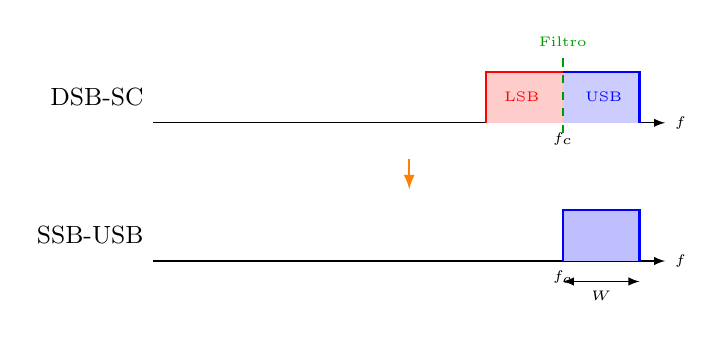
\begin{tikzpicture}[>=latex, scale=0.65]
% DSB-SC
\begin{scope}[yshift=1.5cm]
\draw[->] (-5,0) -- (5,0) node[right, font=\tiny] {$f$};
\fill[red!20] (1.5,0) -- (1.5,1) -- (3,1) -- (3,0) -- cycle;
\fill[blue!20] (3,0) -- (3,1) -- (4.5,1) -- (4.5,0) -- cycle;
\draw[thick, red] (1.5,0) -- (1.5,1) -- (3,1);
\draw[thick, blue] (3,1) -- (4.5,1) -- (4.5,0);
\node[below, font=\tiny] at (3,0) {$f_c$};
\node[font=\tiny, red] at (2.2,0.5) {LSB};
\node[font=\tiny, blue] at (3.8,0.5) {USB};
\node[left, font=\small] at (-5,0.5) {DSB-SC};
\end{scope}
% Filtro
\begin{scope}[yshift=1.5cm]
\draw[thick, green!60!black, dashed] (3,-0.2) -- (3,1.3);
\node[above, font=\tiny, green!60!black] at (3,1.3) {Filtro};
\end{scope}
% Seta
\draw[->, thick, orange] (0,0.8) -- (0,0.2);
% SSB-USB
\begin{scope}[yshift=-1.2cm]
\draw[->] (-5,0) -- (5,0) node[right, font=\tiny] {$f$};
\fill[blue!25] (3,0) -- (3,1) -- (4.5,1) -- (4.5,0) -- cycle;
\draw[thick, blue] (3,0) -- (3,1) -- (4.5,1) -- (4.5,0);
\node[below, font=\tiny] at (3,0) {$f_c$};
\node[left, font=\small] at (-5,0.5) {SSB-USB};
\draw[<->] (3,-0.4) -- (4.5,-0.4) node[midway, below, font=\tiny] {$W$};
\end{scope}
\end{tikzpicture}
\end{center}
}

\only<2>{
\textbf{No tempo (método de Hilbert):}

$m(t)\cos(2\pi f_c t)$ contribui para USB \textbf{e} LSB

$\hat{m}(t)\sin(2\pi f_c t)$ contribui para USB e LSB com \textbf{fases opostas}

\vspace{0.3cm}

\textbf{Combinação que cancela LSB:}
\[
\boxed{s_{\text{USB}}(t) = \frac{A_c}{2}[m(t)\cos(2\pi f_c t) - \hat{m}(t)\sin(2\pi f_c t)]}
\]

O termo $-\hat{m}(t)\sin$ cancela exatamente a LSB, preservando apenas a USB
}

\end{frame}

% ============================================

\begin{frame}{Espectro e Potência do SSB}

\begin{columns}[T]
\begin{column}{0.50\textwidth}
\textbf{Largura de banda:}
\[
\boxed{B_{\text{SSB}} = W}
\]

\onslide<2->{
\textbf{Potência:}
\[
\boxed{P_{\text{SSB}} = \frac{A_c^2 P_m}{4}}
\]

Metade da potência do DSB-SC
}
\end{column}
\begin{column}{0.48\textwidth}
\begin{center}
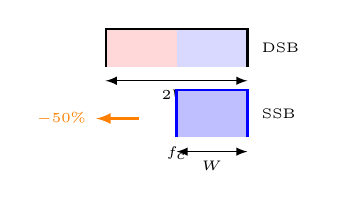
\begin{tikzpicture}[>=latex, scale=0.6]
% DSB-SC
\begin{scope}[yshift=1.5cm]
\fill[red!15] (0.5,0) -- (0.5,0.8) -- (2,0.8) -- (2,0) -- cycle;
\fill[blue!15] (2,0) -- (2,0.8) -- (3.5,0.8) -- (3.5,0) -- cycle;
\draw[thick] (0.5,0) -- (0.5,0.8) -- (3.5,0.8) -- (3.5,0);
\draw[<->] (0.5,-0.3) -- (3.5,-0.3) node[midway, below, font=\tiny] {$2W$};
\node[right, font=\tiny] at (3.6,0.4) {DSB};
\end{scope}
% SSB
\fill[blue!25] (2,0) -- (2,1) -- (3.5,1) -- (3.5,0) -- cycle;
\draw[thick, blue] (2,0) -- (2,1) -- (3.5,1) -- (3.5,0);
\draw[<->] (2,-0.3) -- (3.5,-0.3) node[midway, below, font=\tiny] {$W$};
\node[right, font=\tiny] at (3.6,0.5) {SSB};
\node[below, font=\tiny] at (2,0) {$f_c$};
% Economia
\draw[->, thick, orange] (1.2,0.4) -- (0.3,0.4) node[left, font=\tiny, orange] {$-50\%$};
\end{tikzpicture}
\end{center}

\onslide<2->{
\vspace{0.2cm}
\begin{center}\footnotesize
\begin{tabular}{l c c}
 & DSB-SC & SSB \\
\hline
$B$ & $2W$ & $W$ \\
$P$ & $\frac{A_c^2 P_m}{2}$ & $\frac{A_c^2 P_m}{4}$ \\
\end{tabular}
\end{center}
}
\end{column}
\end{columns}

\end{frame}

% ============================================

\begin{frame}{Geração de SSB: Método do Filtro}

\begin{center}
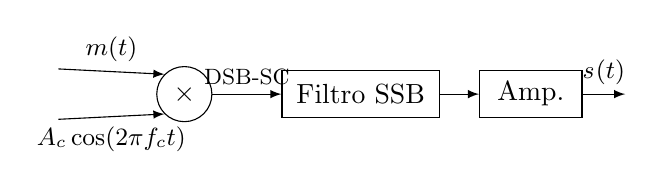
\begin{tikzpicture}[>=latex, scale=0.8]
% Multiplicador
\node[draw, circle, minimum size=0.7cm] (mult) at (0,0) {$\times$};
% Filtro
\node[draw, rectangle, minimum width=2cm, minimum height=0.6cm] (filt) at (2.8,0) {Filtro SSB};
% Amplificador
\node[draw, rectangle, minimum width=1.3cm, minimum height=0.6cm] (amp) at (5.5,0) {Amp.};

% Conexões
\draw[->] (-2,0.4) -- node[above, font=\small] {$m(t)$} (mult.north west);
\draw[->] (-2,-0.4) -- node[below, font=\small] {$A_c\cos(2\pi f_c t)$} (mult.south west);
\draw[->] (mult.east) -- node[above, font=\footnotesize] {DSB-SC} (filt.west);
\draw[->] (filt.east) -- (amp.west);
\draw[->] (amp.east) -- node[above, font=\small] {$s_{\SSB}(t)$} (7,0);
\end{tikzpicture}
\end{center}

\textbf{Processo:}
\begin{enumerate}
\item Gerar DSB-SC: $A_c m(t)\cos(2\pi f_c t)$
\item Filtrar: passa alta de $f_c$ (USB) ou passa baixa de $f_c$ (LSB)
\item Amplificar
\end{enumerate}

\textbf{Desafio:} Filtro deve ter transição abrupta em $f_c$

\end{frame}

% ============================================

\begin{frame}{Geração de SSB: Método de Hilbert}

\begin{center}
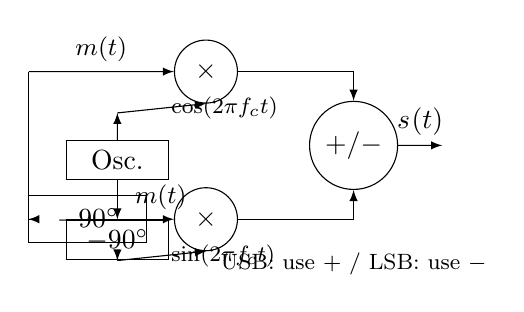
\begin{tikzpicture}[>=latex, scale=0.75]
% Branch superior
\node[draw, circle, minimum size=0.8cm] (mult1) at (2,1.5) {$\times$};
\draw[->] (-1,1.5) -- node[above, font=\small] {$m(t)$} (mult1.west);
\draw[->] (0.5,0.8) -- node[right, font=\footnotesize] {$\cos(2\pi f_c t)$} (mult1.south);

% Branch inferior
\node[draw, rectangle, minimum width=1.5cm, minimum height=0.6cm] (hilb) at (0,-1) {$-90^{\circ}$};
\node[draw, circle, minimum size=0.8cm] (mult2) at (2,-1) {$\times$};
\draw[->] (-1,1.5) |- (hilb.west);
\draw[->] (hilb.east) -- node[above, font=\small] {$\hilbert{m}(t)$} (mult2.west);
\draw[->] (0.5,-1.7) -- node[right, font=\footnotesize] {$\sin(2\pi f_c t)$} (mult2.south);

% Somador
\node[draw, circle, minimum size=0.8cm] (sum) at (4.5,0.25) {$+/-$};
\draw[->] (mult1.east) -| (sum.north);
\draw[->] (mult2.east) -| (sum.south);
\draw[->] (sum.east) -- node[above] {$s_{\SSB}(t)$} (6,0.25);

% Oscilador em fase
\node[draw, rectangle, minimum width=1.3cm, minimum height=0.5cm] (osc) at (0.5,0) {Osc.};
\draw[->] (osc.north) -- (0.5,0.8);
\node[draw, rectangle, minimum width=1.3cm, minimum height=0.5cm] (def) at (0.5,-1.35) {$-90^{\circ}$};
\draw[->] (osc.south) -- (def.north);
\draw[->] (def.south) -- (0.5,-1.7);

% Labels
\node[below of=sum, node distance=1.5cm, font=\footnotesize] {USB: use $+$ / LSB: use $-$};
\end{tikzpicture}
\end{center}

\textbf{Características:}
\begin{itemize}
\item Não requer filtros seletivos
\item Defasador de $-90^{\circ}$ (implementado com all-pass networks)
\item Dois osciladores em quadratura (defasados $90^{\circ}$)
\item Escolha do sinal no somador determina USB ou LSB
\end{itemize}

\textbf{Desafio:} Casamento preciso de amplitude e fase nos dois ramos

\end{frame}

% ============================================

\begin{frame}{Demodulação do SSB}

\only<1>{
\textbf{SSB requer detecção coerente} (como DSB-SC):

\begin{center}
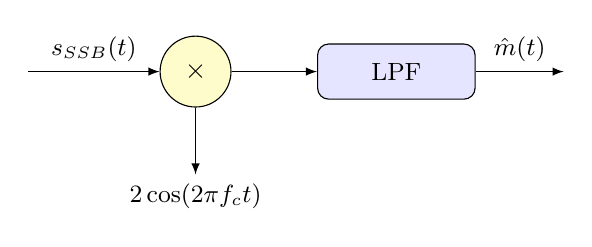
\begin{tikzpicture}[>=latex, scale=0.85]
\node[draw, circle, fill=yellow!20, minimum size=0.9cm] (mult) at (0,0) {$\times$};
\node[draw, rectangle, fill=blue!10, rounded corners, minimum width=2cm, minimum height=0.7cm, font=\small] (lpf) at (3,0) {LPF};
\draw[->] (-2.5,0) -- node[above, font=\small] {$s_{\text{SSB}}(t)$} (mult.west);
\draw[->] (mult.south) -- ++(0,-1) node[below, font=\small] {$2\cos(2\pi f_c t)$};
\draw[->] (mult.east) -- (lpf.west);
\draw[->] (lpf.east) -- node[above, font=\small] {$\hat{m}(t)$} (5.5,0);
\end{tikzpicture}
\end{center}

\vspace{0.2cm}

Com sincronismo perfeito: $\boxed{\hat{m}(t) = m(t)}$
}

\only<2>{
\textbf{Sensibilidade a erro de frequência $\Delta f$:}

Se o oscilador local tem frequência $f_c + \Delta f$:
\[
\hat{m}(t) = m(t) \cos(2\pi\Delta f \cdot t)
\]

\begin{center}
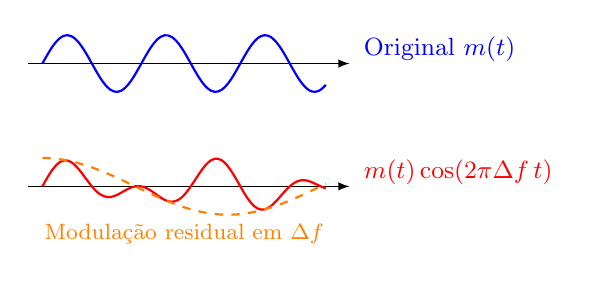
\begin{tikzpicture}[>=latex, scale=0.6]
% Original
\begin{scope}[yshift=1.3cm]
\draw[->] (-0.3,0) -- (6.5,0);
\draw[thick, blue, smooth] plot[domain=0:6, samples=80] (\x, {0.6*sin(3*\x r)});
\node[right, font=\small, blue] at (6.6,0.3) {Original $m(t)$};
\end{scope}
% Com erro
\begin{scope}[yshift=-1.3cm]
\draw[->] (-0.3,0) -- (6.5,0);
\draw[thick, red, smooth] plot[domain=0:6, samples=80] (\x, {0.6*sin(3*\x r)*cos(0.8*\x r)});
\draw[thick, dashed, orange, smooth] plot[domain=0:6, samples=80] (\x, {0.6*cos(0.8*\x r)});
\node[right, font=\small, red] at (6.6,0.3) {$m(t)\cos(2\pi\Delta f\, t)$};
\node[font=\footnotesize, orange] at (3,-1) {Modulação residual em $\Delta f$};
\end{scope}
\end{tikzpicture}
\end{center}

\textbf{Tolerância:} Voz: $\Delta f < 20$ Hz \quad Música: $\Delta f < 2$ Hz
}

\end{frame}

% ============================================

\section{AM VSB}

\begin{frame}{AM VSB: Vestigial Sideband -- A Motivação}

\textbf{Problema com SSB:}

Filtragem abrupta em $f_c$ é difícil, especialmente para sinais com componentes DC ou de muito baixa frequência (ex: vídeo).

\vspace{0.3cm}

\begin{center}
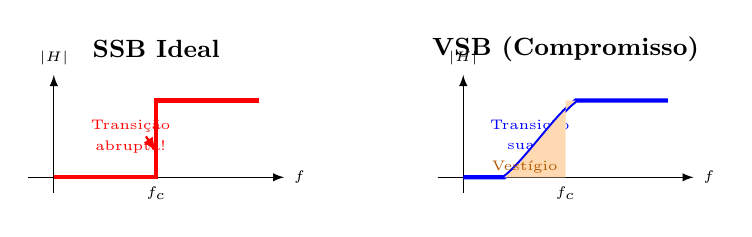
\begin{tikzpicture}[>=latex, scale=0.65]
% SSB ideal
\begin{scope}[xshift=-5cm]
\node[font=\small\bfseries] at (2,2.5) {SSB Ideal};
\draw[->] (-0.5,0) -- (4.5,0) node[right, font=\tiny] {$f$};
\draw[->] (0,-0.3) -- (0,2) node[above, font=\tiny] {$|H|$};
\draw[thick, red, line width=1.5pt] (0,0) -- (2,0) -- (2,1.5) -- (4,1.5);
\node[below, font=\tiny] at (2,0) {$f_c$};
\node[font=\tiny, red] at (1.5,1) {Transição};
\node[font=\tiny, red] at (1.5,0.6) {abrupta!};
\draw[->, red, thick] (1.8,0.8) -- (2,0.5);
\end{scope}

% VSB
\begin{scope}[xshift=3cm]
\node[font=\small\bfseries] at (2,2.5) {VSB (Compromisso)};
\draw[->] (-0.5,0) -- (4.5,0) node[right, font=\tiny] {$f$};
\draw[->] (0,-0.3) -- (0,2) node[above, font=\tiny] {$|H|$};
\draw[thick, blue, line width=1.5pt] (0,0) -- (0.8,0)
    .. controls (1.2,0.3) and (1.8,1.2) ..
    (2.2,1.5) -- (4,1.5);
\node[below, font=\tiny] at (2,0) {$f_c$};
\node[font=\tiny, blue] at (1.3,1) {Transição};
\node[font=\tiny, blue] at (1.3,0.6) {suave};
\fill[orange!30] (0.8,0) .. controls (1.2,0.3) and (1.8,1.2) .. (2.2,1.5) -- (2,1.5) -- (2,0) -- (0.8,0);
\node[font=\tiny, orange!70!black] at (1.2,0.2) {Vestígio};
\end{scope}
\end{tikzpicture}
\end{center}

\textbf{VSB:} Transmitir uma banda lateral completa + ``vestígio'' da outra

\begin{itemize}
\item Largura de banda: $W < B_{\VSB} < 2W$
\item Filtro com roll-off gradual em $f_c$ (realizável!)
\end{itemize}

\textbf{Aplicação principal:} TV analógica (NTSC, PAL)

\end{frame}

% ============================================

\begin{frame}{Visualização VSB: Filtro e Comparação Espectral}

\begin{center}
\includegraphics[width=\figFull, trim=0 345bp 0 0, clip]{figures/cap4/am_vsb.pdf}
\end{center}

\textbf{Esquerda:} Resposta do filtro VSB com roll-off gradual.
\textbf{Direita:} Comparação de espectros DSB, SSB e VSB.

\end{frame}

% ============================================

\begin{frame}{Visualização VSB: Simetria e Largura de Banda}

\begin{center}
\includegraphics[width=\figFull, trim=0 0 0 360bp, clip]{figures/cap4/am_vsb.pdf}
\end{center}

\textbf{Esquerda:} A simetria vestigial em torno de $f_c$ garante recuperação sem distorção.
\textbf{Direita:} Economia de banda: DSB (8.4 kHz) $>$ VSB (5.5 kHz) $>$ SSB (4.2 kHz).

\end{frame}

% ============================================

\begin{frame}{Filtro VSB: Condição de Simetria}

\only<1>{
\textbf{Condição para recuperação sem distorção:}
\[
\boxed{H_{\text{VSB}}(f_c + f) + H_{\text{VSB}}(f_c - f) = \text{constante}}
\]

\begin{center}
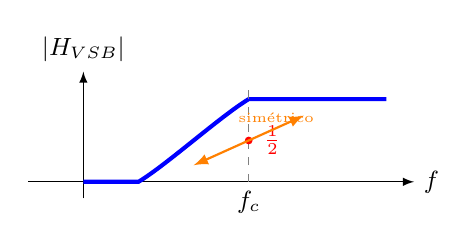
\begin{tikzpicture}[>=latex, scale=0.7]
\draw[->] (-1,0) -- (6,0) node[right, font=\small] {$f$};
\draw[->] (0,-0.3) -- (0,2) node[above, font=\small] {$|H_{\text{VSB}}|$};
% Filtro VSB
\draw[thick, blue, line width=1.5pt] (0,0) -- (1,0)
    .. controls (1.5,0.3) and (2.5,1.2) ..
    (3,1.5) -- (5.5,1.5);
% Linhas de simetria
\draw[dashed, gray] (3,0) -- (3,1.8);
\node[below, font=\small] at (3,0) {$f_c$};
% Ponto de simetria
\fill[red] (3,0.75) circle (2pt);
\node[right, font=\footnotesize, red] at (3.1,0.75) {$\frac{1}{2}$};
% Setas mostrando simetria
\draw[<->, thick, orange] (2,0.3) -- (4,1.2);
\node[above, font=\tiny, orange] at (3.5,0.9) {simétrico};
\end{tikzpicture}
\end{center}

O filtro é simétrico em torno do ponto $\frac{1}{2}$ na frequência $f_c$
}

\only<2>{
\textbf{Sinal VSB:}
\[
s_{\text{VSB}}(t) = [A_c m(t) \cos(2\pi f_c t)] \ast h_{\text{VSB}}(t)
\]

Demodulação coerente + simetria vestigial:
\[
\boxed{y(t) = A_c\, m(t)} \qquad \text{Recuperação perfeita!}
\]

\textbf{Largura de banda:}
\[
\boxed{B_{\text{VSB}} = W + f_{\text{vest}}} \qquad W < B_{\text{VSB}} < 2W
\]

Compromisso entre SSB ($W$) e DSB ($2W$)
}

\end{frame}

% ============================================

\begin{frame}{VSB na TV Analógica (NTSC)}

\only<1>{
\begin{center}
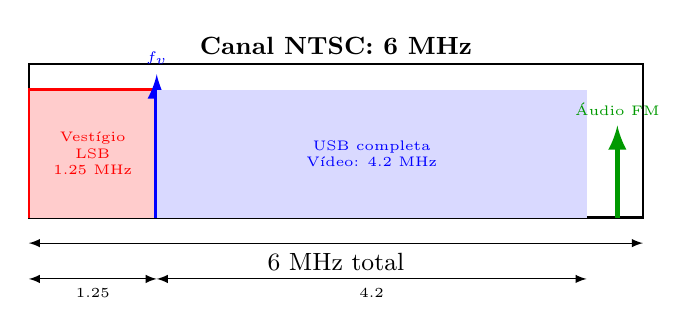
\begin{tikzpicture}[>=latex, scale=0.65]
% Canal de 6 MHz
\draw[thick] (0,0) rectangle (12,3);
\node[above, font=\small\bfseries] at (6,3) {Canal NTSC: 6 MHz};
% Vestígio LSB
\fill[red!20] (0,0) rectangle (2.5,2.5);
\draw[thick, red] (0,0) -- (0,2.5) -- (2.5,2.5) -- (2.5,0);
\node[font=\tiny, red, align=center] at (1.25,1.25) {Vestígio\\LSB\\1.25 MHz};
% Portadora visual
\draw[thick, blue, ->, line width=2pt] (2.5,0) -- (2.5,2.8);
\node[above, font=\tiny, blue] at (2.5,2.8) {$f_v$};
% USB completa (vídeo)
\fill[blue!15] (2.5,0) rectangle (10.9,2.5);
\node[font=\tiny, blue, align=center] at (6.7,1.25) {USB completa\\Vídeo: 4.2 MHz};
% Portadora de áudio FM
\draw[thick, green!60!black, ->, line width=2pt] (11.5,0) -- (11.5,1.8);
\node[above, font=\tiny, green!60!black] at (11.5,1.8) {Áudio FM};
% Medidas
\draw[<->] (0,-0.5) -- (12,-0.5) node[midway, below, font=\small] {6 MHz total};
\draw[<->] (0,-1.2) -- (2.5,-1.2) node[midway, below, font=\tiny] {1.25};
\draw[<->] (2.5,-1.2) -- (10.9,-1.2) node[midway, below, font=\tiny] {4.2};
\end{tikzpicture}
\end{center}
}

\only<2>{
\textbf{Economia de banda:}

\vspace{0.2cm}

\begin{center}
\begin{tabular}{l c c}
 & \textbf{Banda} & \textbf{vs.\ DSB} \\
\hline
DSB & $2 \times 4.2 = 8.4$ MHz & --- \\
VSB (NTSC) & $1.25 + 4.2 = 5.45$ MHz & $-35\%$ \\
SSB ideal & $4.2$ MHz & $-50\%$ \\
\end{tabular}
\end{center}

\vspace{0.3cm}

\textbf{Por que não SSB?}

Sinal de vídeo tem componente DC (nível médio de brilho) $\rightarrow$ filtro abrupto em $f_c$ é impossível

VSB é o \textbf{compromisso prático}: filtro realizável + boa economia de banda
}

\end{frame}

% ============================================

\section{Comparação entre Modulações AM}

\begin{frame}{Tabela Comparativa: Tipos de AM}

\begin{center}
\footnotesize
\begin{tabular}{|l|c|c|c|c|}
\hline
\textbf{Tipo} & \textbf{DSB-SC} & \textbf{AM Conv.} & \textbf{SSB} & \textbf{VSB} \\
\hline
Largura de banda & $2W$ & $2W$ & $W$ & $W<B<2W$ \\
\hline
Potência (relativa) & $1.0$ & $>3.0$ & $0.5$ & $\approx 0.7$ \\
\hline
Eficiência potência & Alta & Baixa & Máxima & Alta \\
& & $(< 33\%)$ & & \\
\hline
Geração & Simples & Simples & Complexa & Moderada \\
\hline
Demodulação & Coerente & Envelope & Coerente & Coerente \\
\hline
Complexidade RX & Média & Mínima & Alta & Média \\
\hline
Sensibilidade $\Delta f$ & Baixa & N/A & Alta & Média \\
\hline
Aplicações & - & Rádio AM & Rádio & TV \\
& & broadcast & amador & analógica \\
\hline
\end{tabular}
\end{center}

\vspace{0.3cm}

\textbf{Escolha depende de:}
\begin{itemize}
\item Largura de banda disponível
\item Potência disponível
\item Complexidade aceitável no TX e RX
\item Custo
\end{itemize}

\end{frame}

% ============================================

\begin{frame}{Comparação Espectral: DSB-SC e AM Convencional}

\begin{center}
\includegraphics[width=\figFull, trim=0 345bp 0 0, clip]{figures/cap4/am_comparison.pdf}
\end{center}

\textbf{DSB-SC:} Apenas bandas laterais, sem portadora.
\textbf{AM Conv.:} Portadora dominante + bandas laterais (maior potência total).

\end{frame}

% ============================================

\begin{frame}{Comparação Espectral: SSB e Sobreposição}

\begin{center}
\includegraphics[width=\figFull, trim=0 0 0 360bp, clip]{figures/cap4/am_comparison.pdf}
\end{center}

\textbf{SSB-USB:} Apenas uma banda lateral (metade da banda).
\textbf{Sobreposição:} Comparação direta dos três esquemas no mesmo gráfico.

\end{frame}

% ============================================

\begin{frame}{Comparação Radar: Variantes AM}

\begin{center}
\includegraphics[width=0.5\textwidth]{figures/cap4/am_radar_comparison.pdf}
\end{center}

\textbf{Cada variante tem seus pontos fortes e fracos} -- a escolha depende da aplicação.

\end{frame}

% ============================================

\begin{frame}{Comparação Espectral Visual}

\begin{center}
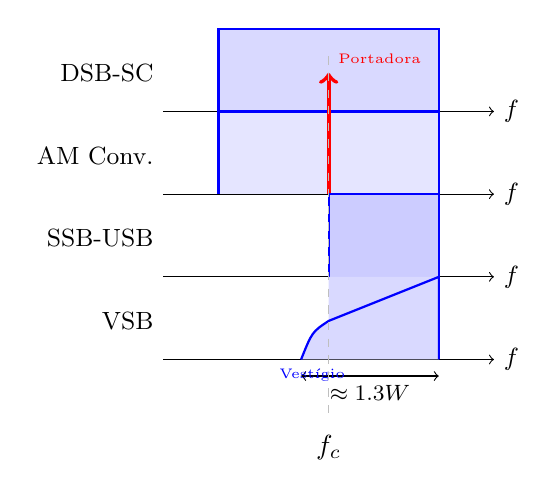
\begin{tikzpicture}[scale=0.7]
% DSB-SC
\begin{scope}[yshift=3cm]
\draw[->] (-3,0) -- (3,0) node[right, font=\small] {$f$};
\fill[blue!15] (-2,0) -- (-2,1.5) -- (2,1.5) -- (2,0) -- cycle;
\draw[thick, blue] (-2,0) -- (-2,1.5) -- (2,1.5) -- (2,0);
\node[left, font=\small] at (-3,0.7) {DSB-SC};
\draw[<->] (-2,-0.3) -- (2,-0.3) node[midway, below, font=\footnotesize] {$2W$};
\onslide<1->{}
\end{scope}

% AM Convencional
\onslide<2->{
\begin{scope}[yshift=1.5cm]
\draw[->] (-3,0) -- (3,0) node[right, font=\small] {$f$};
\fill[blue!10] (-2,0) -- (-2,1.5) -- (2,1.5) -- (2,0) -- cycle;
\draw[thick, blue] (-2,0) -- (-2,1.5) -- (2,1.5) -- (2,0);
\draw[thick, red, ->, line width=1.5pt] (0,0) -- (0,2.2);
\node[left, font=\small] at (-3,0.7) {AM Conv.};
\node[above right, red, font=\tiny] at (0,2.2) {Portadora};
\end{scope}
}

% SSB
\onslide<3->{
\begin{scope}[yshift=0cm]
\draw[->] (-3,0) -- (3,0) node[right, font=\small] {$f$};
\fill[blue!20] (0,0) -- (0,1.5) -- (2,1.5) -- (2,0) -- cycle;
\draw[thick, blue] (0,0) -- (0,1.5) -- (2,1.5) -- (2,0);
\node[left, font=\small] at (-3,0.7) {SSB-USB};
\draw[<->] (0,-0.3) -- (2,-0.3) node[midway, below, font=\footnotesize] {$W$};
\end{scope}
}

% VSB
\onslide<4->{
\begin{scope}[yshift=-1.5cm]
\draw[->] (-3,0) -- (3,0) node[right, font=\small] {$f$};
\fill[blue!15] (-0.5,0) .. controls (-0.3,0.5) .. (0,0.7) -- (0,1.5) -- (2,1.5) -- (2,0) -- cycle;
\draw[thick, blue] (-0.5,0) .. controls (-0.3,0.5) .. (0,0.7)
                   -- (2,1.5) -- (2,0);
\node[left, font=\small] at (-3,0.7) {VSB};
\draw[<->] (-0.5,-0.3) -- (2,-0.3) node[midway, below, font=\footnotesize] {$\approx 1.3W$};
\node[below, blue, font=\tiny] at (-0.3,0) {Vestígio};
\end{scope}
}

% fc marca
\draw[dashed, gray!50] (0,4) -- (0,-2.5);
\node[below] at (0,-2.7) {$f_c$};
\end{tikzpicture}
\end{center}

\end{frame}

% ============================================

\begin{frame}{Aplicações Práticas das Variantes AM}

\begin{columns}[T]
\begin{column}{0.48\textwidth}
\onslide<1->{
\textbf{AM Convencional:}
\begin{itemize}
\item Rádio AM (535--1705 kHz)
\item Receptor barato (envelope)
\end{itemize}
}

\onslide<2->{
\vspace{0.2cm}
\textbf{DSB-SC:}
\begin{itemize}
\item Estéreo FM (sinal L$-$R)
\item Cor em TV (QAM)
\end{itemize}
}
\end{column}
\begin{column}{0.50\textwidth}
\onslide<3->{
\textbf{SSB:}
\begin{itemize}
\item Rádio amador (HF: 3--30 MHz)
\item Marítima, aeronáutica, militar
\end{itemize}
}

\onslide<4->{
\vspace{0.2cm}
\textbf{VSB:}
\begin{itemize}
\item TV analógica (NTSC, PAL)
\item TV digital (ATSC)
\end{itemize}
}
\end{column}
\end{columns}

\onslide<5->{
\vspace{0.3cm}

\textbf{Escolha depende de:} banda disponível, potência, custo do receptor, tipo de sinal
}

\end{frame}

% ============================================

\begin{frame}{Resumo: Modulação em Amplitude}

\textbf{Conceitos fundamentais:}
\begin{itemize}
\item Modulação desloca espectro de banda base para RF
\item Facilita multiplexação, propagação e processamento
\end{itemize}

\vspace{0.3cm}

\textbf{Quatro variantes principais:}

\begin{enumerate}
\item \textbf{DSB-SC:} $s(t) = A_c m(t)\cos(2\pi f_c t)$
   \begin{itemize}
   \item Simples, mas requer detecção coerente
   \end{itemize}

\item \textbf{AM Convencional:} $s(t) = A_c[1 + k_a m(t)]\cos(2\pi f_c t)$
   \begin{itemize}
   \item Detector de envelope, mas ineficiente ($\eta \leq 33\%$)
   \end{itemize}

\item \textbf{SSB:} Usa transformada de Hilbert
   \begin{itemize}
   \item Economiza largura de banda (50\%)
   \end{itemize}

\item \textbf{VSB:} Compromisso DSB-SSB
   \begin{itemize}
   \item Ideal para sinais com componentes DC/baixa frequência
   \end{itemize}
\end{enumerate}

\textbf{Escolha baseada em:} Banda disponível, potência, complexidade, custo

\end{frame}
